\documentclass[relqm.tex]{subfiles}

\begin{document}
\part{Particle Physics Phenomenology}
\chapter{A Brief History...}
The modern outlook of particle physics is based on these elementary particles:
\textit{draw table of all particles}
Back in the 1940s, we did not have the same scope. 
We knew about protons, neutrons, and electrons. 
Then we discovered pions and muons coming in from the atmosphere, using cloud chambers and their difference of decay rate to distinguish them.
So we added the muon to our elementary particles.
Pions hinted towards the existence of quarks, made of u and d quarks.

\section{...of QCD}
\begin{itemize}
    \item Not long after, we discovered the Kaon as well. 
        We saw something decay into two pions which had to be heavier. 
        Kaons contain the s quark, so lead eventually to the higher generations of quarks. 
    \item Over time, more particles were slowly discovered, e.g. myriads of mesons like $\pi$, K, $\rho$, $\eta$, etc. 
    \item Gell-Mann realised that all these particles we were finding could be made up of more elementary particles called quarks, with different combinations and numbers yielding the different particles we knew at this time.
        There was no evidence at this time that this would be the case, it was just a useful thought experiment. 
    \item In the late 60s, the Stanford accelerator used deep inelastic scattering to decompose the proton and resolve its constituents, i.e. the parton model leading to confirmation of quarks.
    \item Gell-Mann and others fledge out their theory of quarks into a full gauge theory into what we know today as SU(3) QCD.
        This was ultimately confirmed when the $J/\Psi$ ($c\bar{c}$) was discovered by two separate accelerators, so now the quark model for the first two generations was found and made sense of the current catalogue of composite particles.
    \item Shortly after, we found experimental confirmation of the gluon, making sense of quarks as a gauge theory. 
    \item We then discovered the $\Upsilon$ ($b\bar{b}$) meson in the mid 70s, which hinted at a third generation of quarks, but the top quark was to remain elusive until \~95.
\end{itemize}

\section{...of GSW Theory}
\begin{itemize}
    \item In the mid 50s, we found interactions between protons and neutrinos to form neutrons and leptons, both for first and second generation.
    \item We required the same number of generations of quarks and leptons, and slowly we found the third generation of leptons by 2000 with the discovery of $\nu_\tau$.
    \item The interactions with neutrinos studied hinted to some other interaction besides electromagnetism and QCD, with its strength described in the Fermi constant. 
        These interactions all seemed pointlike to us as the particle mediating them was so much heavier than the others. 
    \item Glashow et al formed this into a gauge theory to attempt to describe this, finding the $W^\pm,Z$ bosons, as well as combining this with the electromagntic gauge theory to form the electroweak of SU(2)$\times$U(1).
    \item In the 1980s at CERN, electrons and positrons were collided to produce the $W^\pm,Z$ bosons and measured their masses as \~80 and 90 GeV respectively, values which were predicted back in the 60s by Weinberg and Salam.
\end{itemize}

\section{...of the Higgs theory}
\begin{itemize}
    \item The big issue we had was that all our theories worked on gauge invariance which would be broken by mass terms to form the masses we knew these particles had. 
    \item Many people postulated what we now know as the Higgs mechanism at roughly the same time, in the 60s. 
    \item Very skeptical for many years about this theory, although it was seen as the simplest way to get it done. 
        Then in 2012, CERN found what we believe to be the Higgs boson, completing the current picture of particle physics, encompassing all forces, interactions, and particles predicted by the Standard Model.
\end{itemize}

\section{Some Notes on Notation and Terminology}
\begin{itemize}
    \item Pions, Kaons, and any other particles made of one quark and an anti-quark are known as \textbf{Mesons}.
    \item Neutrons, protons, and other three-quark particles are known as \textbf{Baryons}.
    \item Overall, any particle made of quarks is called a \textbf{Hadron}.
    \item Leptons never really form bound states until electrons are bound by atoms, so there is not much terminology for them. 
\end{itemize}
Next time, we will discuss particle colliders and their two parameters, COM energy and Luminosity. 
Collider physics is governed by the rate of events,
\begin{equation}
    \frac{dN_{ev}}{dt} = L\sigma,
\end{equation}
where $L$ is luminosity and $\sigma$ is the cross-section.

\chapter{The LHC}
Collisions between two particles are the basis for experimental particle physics. 
Particles have four -momenta $p=(E_p,\vp)$, where the total four-momenta going in will be $p_T=(E_1+E_2,\vp_1+\vp_2)$.
We can transform between coordinate systems of our four-momenta as
\begin{align}
    \frac{1}{\sqrt{1-v^2}}\begin{pmatrix}1& -\vv \\ -\vv & 1\end{pmatrix}\begin{pmatrix} E_1 \\ \vp_1\end{pmatrix} &= \frac{1}{\sqrt{1-v^2}}\begin{pmatrix} E_1-\vv\vp_1 \\ -\vv E_1 - p_1\end{pmatrix} \\
                                          &= \tensor{\Lambda}{_\mu^\nu}p_\nu
\end{align}
We can choose the simplest frame for this, i.e. the COM frame:
\begin{align}
    (p_1+p_2)_{cm} &= \begin{pmatrix} E_1^{cm} + E_2^{cm} \\ 0 \end{pmatrix} \\
    \frac{1}{\sqrt{1-v^2}}\begin{pmatrix}1& -\vv^{cm} \\ -\vv^{cm} & 1\end{pmatrix}\begin{pmatrix} E_1 + E_2 \\ \vp_1 + \vp_2\end{pmatrix} &= \frac{1}{\sqrt{1-v^2}}\begin{pmatrix} E_1 + E_2 -\vv^{cm}(\vp_1+\vp_2) \\ -\vv^{cm}( E_1+E_2) - \vp_1-\vp_2\end{pmatrix}  \\
    s = (E_1^{cm}+E_2^{cm})^2 &= (p_1+p_2)^\mu(p_1+p_2)_\mu = (E_1+E_2)^2 - (\vp_1+\vp_2)^2
\end{align}
The LHC currently has a COM energy of 13 TeV, i.e. during proton-proton collisions, each proton as $E_p=6.5\,$TeV, with three-momenta equal in magnitude with opposite signs. 
Consider proton at rest ($p_1=(m_p,0)$) colliding with electron ($p_2=(E_2,\vp_2)$):
\begin{align}
    s = (p_1+p_2)^2 &= (m_p+E_2)^2 = m_p^2 + 2E_2m_p + \underbrace{E_2^2-p_2^2}_{m_e^2} \\
    E_{cm} = \sqrt{s} &= 100\,\text{GeV}
\end{align}
So we switched from fixed targets to two moving targets as it massively increases COM energy available, although we will see that not all this energy is the energy available for particle production. 
We consider the cross-section concept for proton collisions, where
\begin{align}
    \frac{dN_{ev}}{dt} &= 2vn_2N_1\sigma = L\times\sigma,
\end{align}
so the number of events occuring is dependent on the cross-section of the beams.
We have defined $L$ as the instantaneous \emph{luminosity}, which is like flux in astronomy etc. 
So the number of events is dependent on the cross-section of beam collisions and the how often particles are included within the cross-section (in the Luminosity).
We can describe each of the particles in these collisions using a Gaussian profile density of form
\begin{align}
    \rho &= \exp\left(-\frac{x^2}{2\,dx^2}-\frac{y^2}{2\,dy^2}-\frac{z^2}{2\,dz^2}\right).
\end{align}
We can then write the Luminosity as
\begin{align}
    L &= \frac{fN_1N_2N_b}{4\pi\,dx\,dy}.
\end{align}
We do not have a continuous beam of particles in these colliders, but a small collection of beams, where there will be $N_b$ travelling in each direction.
The Luminosity of the LHC is $L_{int}=140\,\text{fb}^{-1}$, where fb is defined as femtobarn ($1\,$fb $=10^{-15}\,$b $=10^{-39}\,$cm$^2$).
If we consider the cross-section of proton collisions for Higgs production, $\sigma_{pp\to h}=4\times10^4\,$fb, we can calculate the number of Higgs produced at the LHC as $N_{h}=5.6\times10^6$.

\section{The CMS detector at CERN}
\begin{figure}[H]
    \centering
    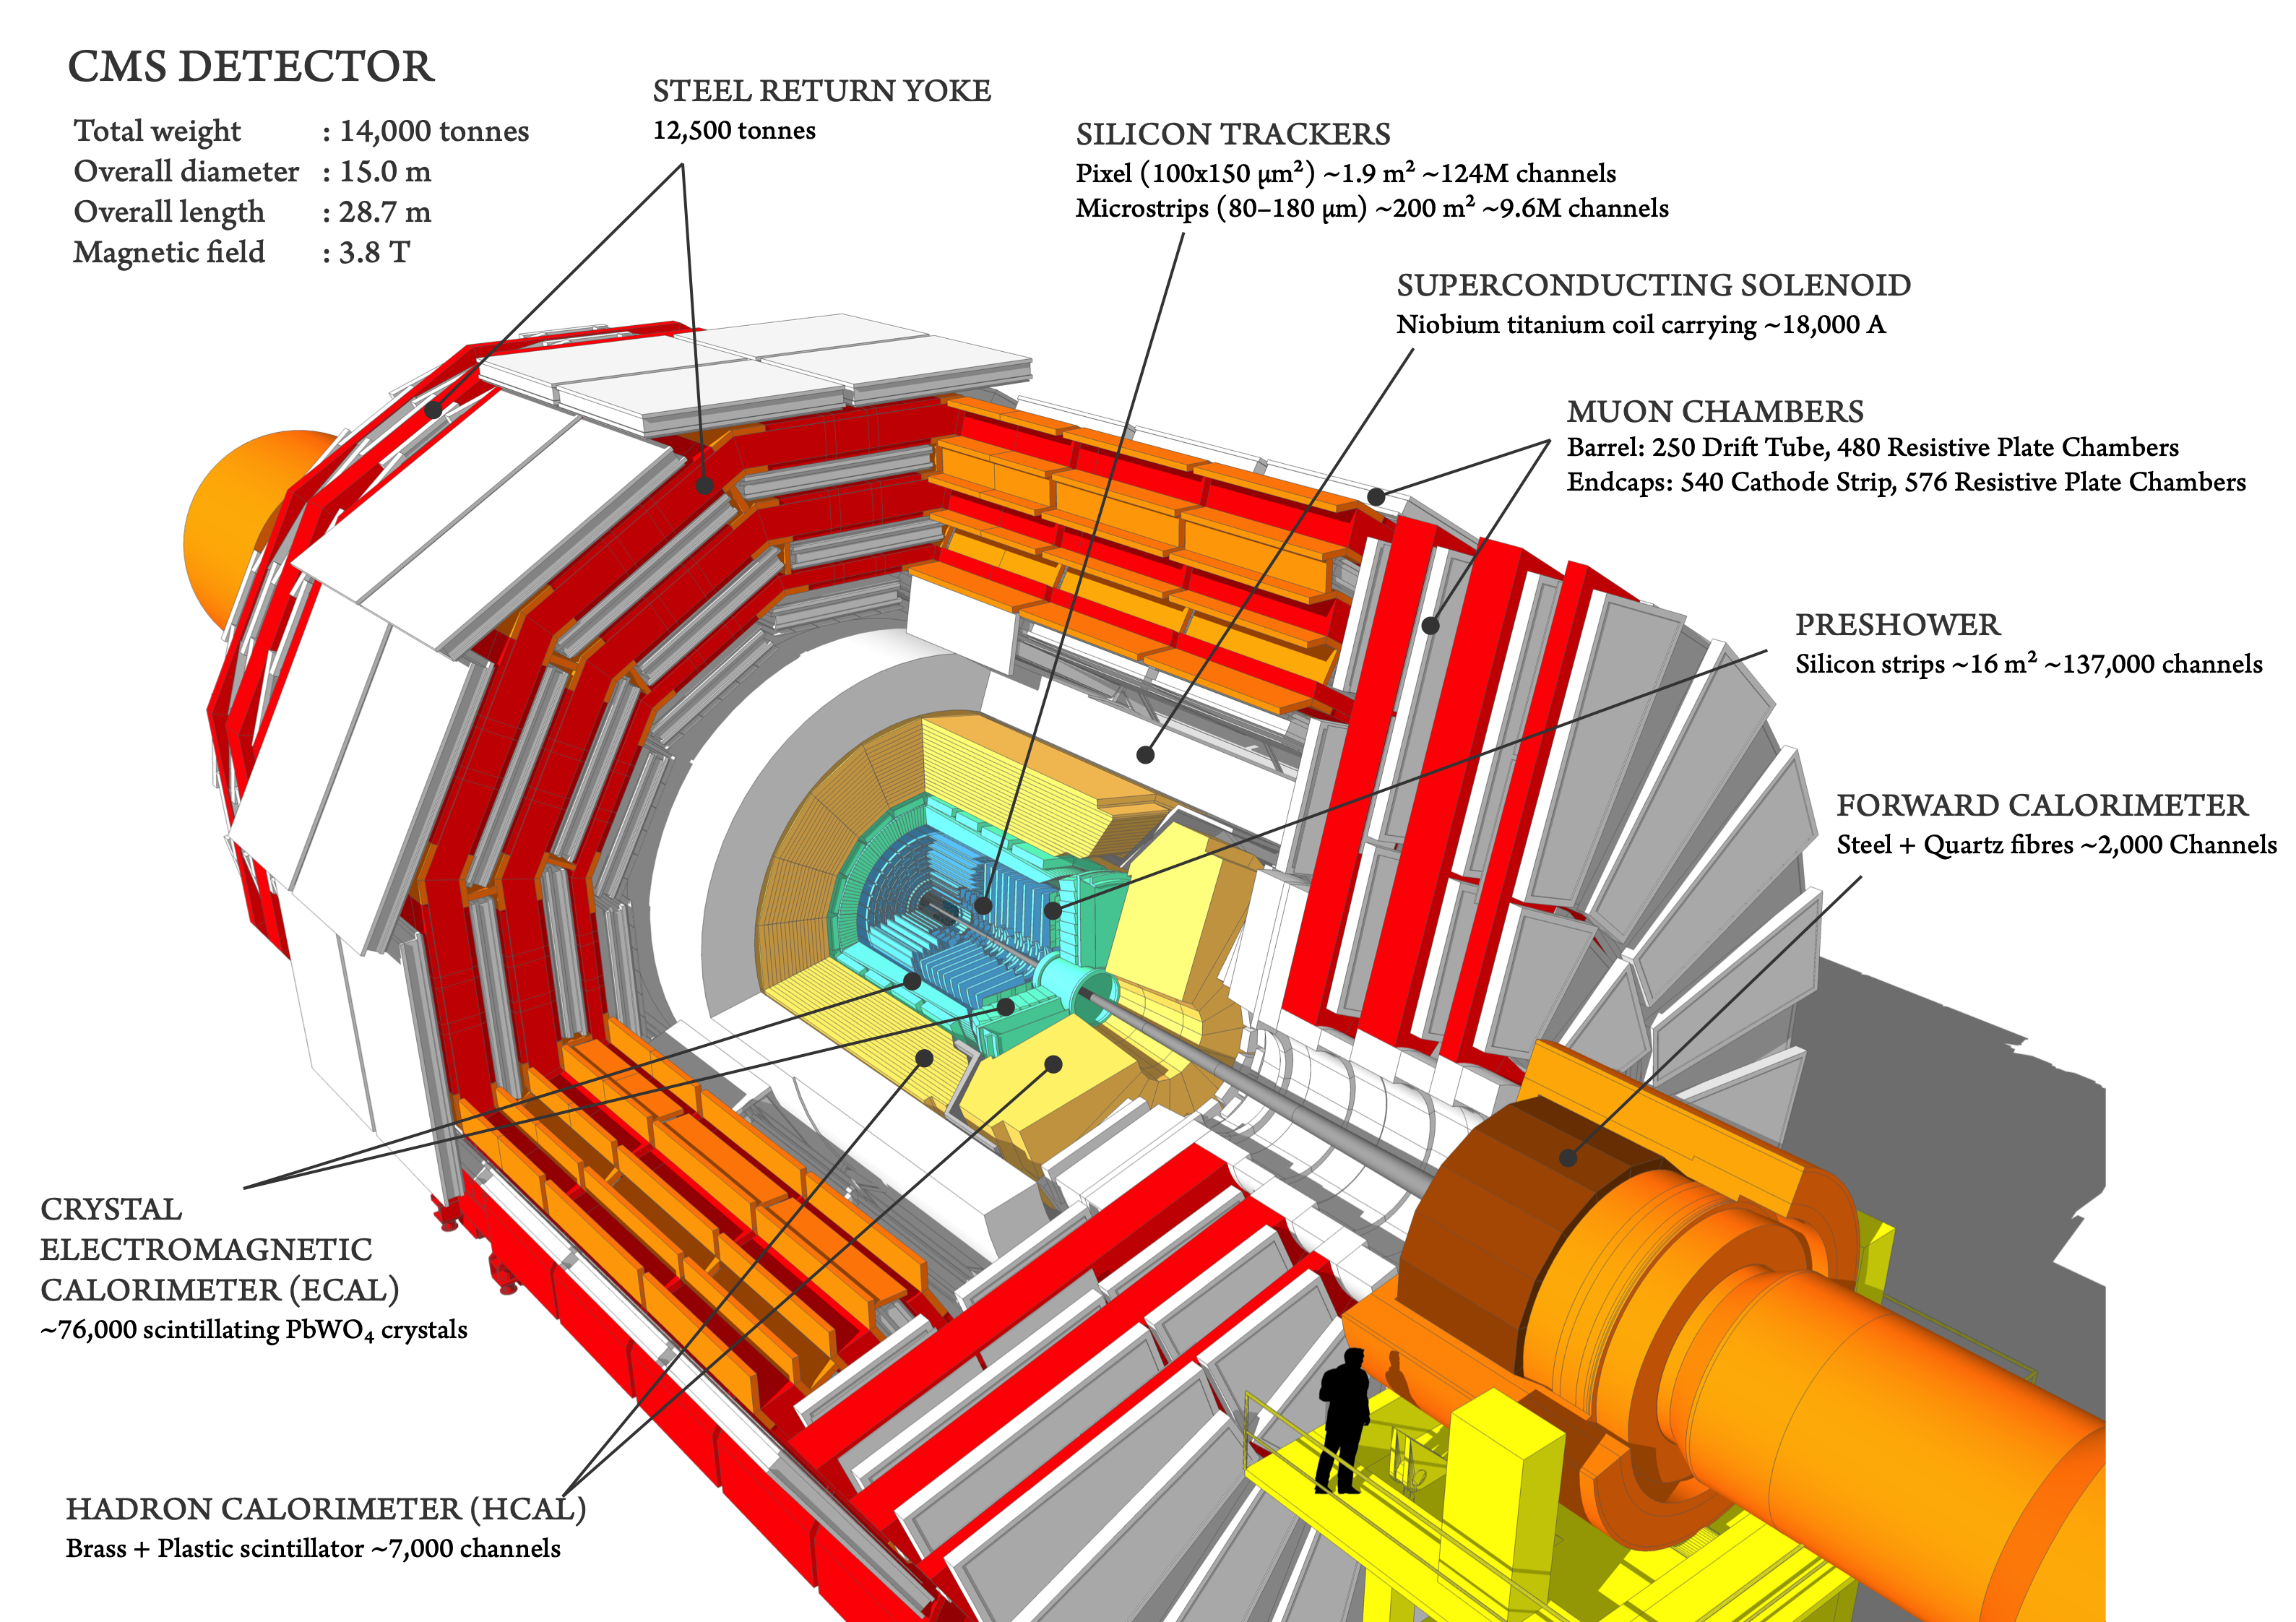
\includegraphics[width=0.9\textwidth]{CMS_160312_06.png}
\end{figure}
\begin{itemize}
    \item CMS (Compact Muon Solenoid) is a 14000 ton experiment, $15\times15$m$^2$.
    \item We have a ``tracker" made out of silicon which tracks the particles, as charged particles' paths are bent moving through it due to the magnetic field generated by the surrounding superconductor.
    \item The particles will then collide into a ``electromagnetic calorimeter" which allows us to measure their energy if they are electrons. 
    \item There is then a ``hadron calorimeter" which will collide with hadrons, i.e. pions, and measure their energy. 
    \item Finally there is a muon chamber, which of course detects muons.
    \item Neutrinos will not be detected by any of these chambers, but we can infer if one has been produced through the starting energy/masses and the measured outputs of electrons, hadrons, and muons. 
        Other low-interacting particles could be present in this as well, but so far all scattering events observed have been consistent with the missing particles being neutrinos.
\end{itemize}
We write length in units of $\frac{1}{\text{GeV}}$, which makes sense, when you multiply by $\hbar c$ and propagate through, it is then in units of approximately $2\times10^{-16}$m.
This length scale will explain why we do not observe quarks on their own - they hadronise in a shorter time than it takes for us to observe them. 
Top quarks can however be observed on their own as their lifetime is shorted than the hadronisation time due to their significant mass, $m_t=172.9\,$GeV.

\chapter{Path Integrals and Feynman Rules}
Consider a quantum system with our conjugate operators $\hat{Q}$ and $\hat{P}$. 
These satisfy the familiar defintions:
\begin{align}
    [\hat{Q},\hat{P}] &= i\hbar & \hat{Q}|Q\rangle &= Q|Q\rangle \\
    \langle Q|P|\rangle &= e^{iQP/\hbar} & \hat{P}|P\rangle &= P|P\rangle.
\end{align}
We can now consider the time evolution of the system using the time-dependent Schrodinger equation,
\begin{align}
    i\hbar\dpt|Q(t)\rangle &= \Ham, & \Ham &= \frac{\hat{P}^2}{2} + V(\hat{Q}).
\end{align}
We consider a non-relativistic object moving in one dimension with unit mass $M=1$.
The amplitude is therefore
\begin{align}
    \langle Q_F|e^{-i\Ham T/\hbar}|Q_I\rangle.
\end{align}
We break the time $T$ into $N+1$ intervals, such that $\delta t = T/(N+1)$, and evaluate the operators in terms of eigenvalues using several identities. 
\begin{align}
    \langle Q_F|e^{-i\Ham T/\hbar}|Q_I\rangle &= \langle Q_F|e^{-i\Ham \delta t/\hbar}\dots e^{-i\Ham \delta/\hbar}|Q_I\rangle \\
                                              &= \int \langle Q_F|e^{-i\Ham \delta t/\hbar}|Q_{N-1}\rangle\dots\langle Q_2|e^{-i\Ham\delta t/\hbar}|Q_1\rangle\langle Q_1|e^{-i\Ham\delta t/\hbar}|Q_I\rangle\prod_i dQ_i.
\end{align}
We can break down each product of this:
\begin{align}
    \langle Q_{j+1}|e^{-i\Ham\delta t/\hbar}|Q_j\rangle &= \int \langle Q_{j+1}|e^{-i\Ham\delta t/\hbar}|P\rangle\langle P|Q_j\rangle\frac{dP}{2\pi} \\
                                                        &= \int \langle Q_{j+1}|P\rangle e^{-i\frac{\delta t}{\hbar}(\frac{P^2}{2}+V(i\hbar\frac{\p}{\p P}))}\langle P|Q_j\rangle\frac{dP}{2\pi} \\
    &= \int e^{i\frac{Q_{j+1}P}{\hbar}}e^{-i\frac{\delta t}{\hbar}(\frac{P^2}{2}+V(i\hbar\frac{\p}{\p P}))}e^{-i\frac{Q_jP}{\hbar}}\frac{dP}{2\pi}.
\end{align}
The argument of the exponential is then:
\begin{align}
    -\frac{i\delta t}{\hbar}\left(\frac{P^2}{2}-\frac{P}{\delta t}(Q_{j+1}-Q_j)+V(Q_j)\right) &= -\frac{i\delta t}{\hbar}\left(\frac12\left(P - \frac{Q_{j+1}-Q_j}{\delta t}\right)^2 - \frac{(Q_{j+1}-Q_j)^2}{2\delta t^2} + V(Q_j)\right).
\end{align}
We can see that the integral in P is Gaussian which in general yields
\begin{align}
    \ifnt \exp\left(-\frac{(z-b)^2}{2a^2}\right)\,dz &= \sqrt{2\pi a^2},
\end{align}
so therefore the integral in P is
\begin{align}
    \int \langle Q_{j+1}|e^{-i\frac{\Ham\delta t}{\hbar}}|P\rangle\langle P|Q_j\rangle\frac{dP}{2\pi} &= \sqrt{\frac{\hbar}{i2\pi\delta t}}\exp\left[\frac{i\delta t}{\hbar}\left(\frac{(Q_{j+1}-Q_j)^2}{2\delta t^2} - V(Q_j)\right)\right].
\end{align}
The amplitude now reads
\begin{align}
    \begin{split}
        \langle Q_F|e^{-\frac{i}{\hbar}\Ham T}|Q_I\rangle = \left(\frac{-i\hbar}{2\pi\delta t}\right)^{\frac{N+1}{2}} \int \prod_j &\left\{\exp\left[\frac{i\delta t}{\hbar}\left(\frac{(Q_{j+1}-Q_j)^2}{2\delta t^2}-V(Q_j)\right)\right]\,dQ_j\right\} \\
                                                                                                                                   &\times \exp\left[\frac{i\delta t}{\hbar}\left(\frac{(Q_1-Q_I)^2}{2\delta t^2}-V(Q_I)\right)\right].
    \end{split}
\end{align}
with $Q_{N+1}=Q_F$.
We can then write the infintesimal limit of $\delta t\to0$ to get
\begin{align}
    \langle Q_F|Q_I\rangle &= \int_{Q_I}^{Q_F} \mathcal{D}Qe^{-\frac{i}{\hbar}S[Q]}, \text{ where }\\
    S[Q] &= \int_0^T \La(Q)\,dt = \int_0^T \left(\frac{\dot{Q}^2}{2}-V(Q)\right)\,dt, \\
    \mathcal{D}Q &= \lim_{\delta t\to0} \left(\frac{-i\hbar}{2\pi\delta t}\right)^{\frac{N+1}{2}}\prod_i dQ_i.
\end{align}
We call $S[Q]$ the \emph{action}, from which we can arrive at the Euler-Lagrange equations where $\frac{\delta S[Q]}{\delta Q} = 0$.
So we sum over all paths and it is the action that determines the final results, the evolutions of the sytem. 
From here already one can see the importance of the action and Lagrangian. Finding the fundamental action that describes the world is key to predict and understand the possible outcomes. 
This makes the case for theorists to fixate with Lagrangians: there is the hope that the search for new phenomena will yield a complex description of Nature as specified by the Action. 

Now we can connect to particle physics by
\begin{align}
    Q &\to \phi(t,\vx), & P &\to \p_t\phi(t,\vx) = \Pi, 
\end{align}
where we can now define our Lagrangian as
\begin{align}
    \La &= \frac12 \p_\mu\phi\p^\mu\phi - m^2\phi^2. 
\end{align}
The commutation relation can be defined as
\begin{align}
    [\hat{\phi}(\vx),\hat{\Pi}(\vec{y})] &= i\hbar\delta^3(\vx-\vec{y}).
\end{align}
We have a Hamiltonian and Action from these, reading
\begin{align}
    \Ham &= \frac{\p_t\hat{\phi}^2}{2} + \frac12\left(\del\hat{\phi}\right)^2+V(\hat{\phi}), \\
    S[\phi] &= \int \left(\frac12\p_\mu\phi\p^\mu\phi - V(\phi)\right)\,dt\,dt^3\vx.
\end{align}
From here, we can build up our rules as previously, but we would only get a number of single-particles states. 
For this to be a description of nature, we need multi-particle states as well. 
To this end, we introduce the partition function:
\begin{align}
    Z[0] &= \langle0|e^{-\frac{i}{\hbar}\Ham T}|0\rangle_{T\to\infty} = \int\mathcal{D}e^{iS[\phi]}\\
    Z[J] &= \int \mathcal{D}\phi\exp\left[iS[\phi]+i\int\phi(x)J(x)\,d^4x\right].
\end{align}

\chapter{Path Integrals and Feynman Rules, Contd.}
From the scalar action of Eq. (3.21) and the two-point correlator,
\begin{align}
    \frac{\delta^2}{i\delta J(x)i\delta I(y)}\frac{Z[J]}{Z[0]}\bigg|_{j=0} &= \frac{1}{Z[0]}\int \mathcal{D}\phi(x)\phi(y)e^{iS[\phi]},
\end{align}
where functional derivatives are defined by
\begin{align}
    \frac{\delta J(y)}{\delta J(x)} &= \delta^4(x-y).
\end{align}
Now we can rewrite the action as
\begin{align}
    \int \left(\frac12\phi(-\Box-m^2)\phi+\phi J\right)\,d^4x &= \in \left(\frac12(\phi+\Delta J)(-\Box-m^2)(\phi+\Delta J) - \frac12 J\Delta J\right)\,d^4x\\
                                                              &= \int \left(\frac12\tilde{\phi}(-\Box-m^2)\tilde{\phi} - \frac12 J\Delta J\right)\,d^4x,
\end{align}
using integration by parts with $\Box=\p^\mu\p_\mu$.
Here, $\Delta = (-\Box-m^2)^{-1}$, and $\tilde{\phi}=\phi+\Delta J$.
This result back in the path integral gives
\begin{align}
    \frac{1}{Z[0]}\int \mathcal{D}\tilde{\phi}e^{i\S[\tilde{\phi}]}\frac{\delta^2}{i^2\delta J^2}e^{-\frac{i}{2}\int J\Delta J}\bigg|_{J=0} &= \left(i\Delta + (\Delta J)^2\right)e^{\frac{i}{2}\int J\Delta J}\bigg|_{J=0} = i\Delta,
\end{align}
where we have identified the path integral in $\tilde{\phi}$ as $Z[0]$.
Specifically,
\begin{align}
    (-\Box-m^2)(\Delta J)(x) &= (-\Box-m^2)\int \Delta(x,y)J(y)\,d^4y, \\
    \Delta(x,y) &= \int \frac{e^{iq(x-y)}}{q^2-m^2}\frac{d^4q}{(2\pi)^4}.
\end{align}
So all we had to do to compute the integral is to invert the operator of the quadratic action in $\phi$.
We obtain the propagation of a field from $x$ to $y$ in the absence of interactions, but now we want to include these. 
We can study the scattering matrix $S$, computed from the path integral for $N$ particles as
\begin{align}
    S &= \frac{1}{Z[0]}\left((i\Delta)^{-1}\frac{\delta}{i\delta J}\right)^NZ[J]\bigg|_{J=0} = \frac{1}{Z[0]}\left((i\Delta)^{-1}\frac{\delta}{i\delta J}\right)^N \int \mathcal{D}\phi e^{iS[\phi]+\int J\phi}\bigg|_{J=0} \\
      &= \frac{1}{Z[0]}\int \mathcal{D}\tilde{\phi}e^{iS_0[\tilde{\phi}]}\left((i\Delta)^{-1}\frac{\delta}{i\delta J}\right)^N \exp\left[-\frac{i}{2}\int J\Delta J + iS_{int}[\tilde{\phi}-\Delta J]\right]\bigg|_{J=0} \\
      &= \frac{1}{Z[0]}\int \mathcal{D}\tilde{\phi}e^{iS_0[\tilde[\phi]-\frac{i}{2}\int J\Delta J} \left((i\Delta)^{-1}\frac{\delta}{i\delta J}\right)^N e^{iS_{int}[\tilde{\phi}-\Delta J]}+\text{ disconnected} \\
      &= \frac{1}{Z[0]}\int \mathcal{D}\phi e^{iS_0[\phi]}\left(\frac{\delta}{\delta\phi(p)}\right)^Ne^{iS_{int}[\phi]}+\text{ disconnected}.
\end{align}
This is the \textbf{Lehmann Symanzyk Zimmerman} reduction formula and there is a lot to unpack. 
The disconnected terms are best understand with a diagrammatic approach:
\begin{figure}[H]
    \centering
    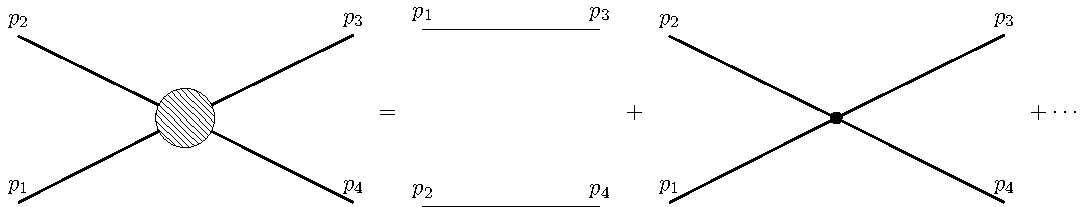
\includegraphics[width=0.8\textwidth]{fours.pdf}
\end{figure}
Here we can see the disconnected refers to processes in which some particles travel freely and corresponds to letting $\frac{\delta}{\delta J}$ act on the free piece $\exp\left(-i\int J\Delta J/2\right)$.
To get acquainted with this expression, consider the S matrix for the following interaction:
\begin{align}
    S_{int}[\phi] &= -\int \frac{\lambda}{4!}\phi(x)^4\,d^4x = -\frac{\lambda}{4!}\int d^4x \prod_{i=1}^4 \int e^{ip_ix}\phi(p_i)\,d^4p_i \\
                  &= -\frac{\lambda}{4!}\prod_{i=1}^4 \left[\int \phi(p_i)\,d^4p_i\right](2\pi)^4\delta^4\left(\sum p_i\right).
\end{align}
We consider 2 to 2 particle scattering with incoming momenta $k_1,k_2$ and outgoing momenta $k_3,k_4$.
Now taking the derivative, the out-states have flipped momenta:
\begin{align}
    e^{iS_0[\phi]}\frac{\delta^2}{\delta\phi(k_1)\delta\phi(k_2)}\frac{\delta^2}{\delta\phi(-k_4)\delta\phi(-k_3)}e^{iS_{int}[\phi]} &= e^{iS[\phi]}(-i\lambda)(2\pi)^2\delta(k_1+k_2-k_3-k_4)+\mathcal{O}(\lambda^2),
\end{align}
i.e. the path integral on $e^{iS}$ cancels out with the factor $Z[0]$ in the denominator and we have therefore obtained the first order in $\lambda$ matrix element $S$.
The invariant matrix element is then defined as
\begin{align}
    S &= \Pi - i(2\pi)^4\delta^4(p_I-p_F)\mathcal{M},
\end{align}
where $p_{I,F}$ sum over the initial and final momenta. 
We then find that $-i\mathcal{M}=-i\lambda$.

Now consider the case of a proton with field $P(x)$ scattering off an electron with field $e(x)$ via the electromagnetic interaction:
\begin{align}
    D_\mu P(x) &= (\p_\mu+iQA_\mu)P(x) \\
    S_{int} &= \int \left(Q\bar{e}(x)\gamma_\mu e(x)A^\mu(x) - Q\bar{P}(x)\gamma_\mu P(x)A^\mu(x)\right)\,d^4x.
\end{align}
The $S$ matrix is then computed from
\begin{equation}
    \begin{split}
        &e^{iS_0[e,P,A_\mu]}\frac{\delta}{\delta\bar{e}(p_2)}\frac{\delta}{\delta e(p_1)}\frac{\delta}{\delta\bar{P}(k_2)}\frac{\delta}{\delta P(k_1)}e^{iS_{int}[e,P,A_\mu]} \\
        =&e^{iS[e,P,A_\mu]}\int e^{i(p_1-p_2)x}[iQ\gamma_\mu]A^\mu(x)\,d^4x \int e^{i(k_1-k_2)y}[-iQ\gamma_\nu]A^\nu(y)\,d^4y + \mathcal{O}(Q^4) \\
        =&e^{iS[e,P,A_\mu]-iS_0[A_\mu]}\int d^4x \int e^{i(p_1-p_2)x}(iQ\gamma_\mu)\left[A^\mu(x)A^\nu(y)e^{iS_0[A_\mu]}\right]e^{i(k_1-k_2)y}(-iQ\gamma_\nu)\,d^4y.
    \end{split}
\end{equation}
We can perform the path integral in $A_\mu$ perturbatively and yield precisely the propagator
\begin{equation}
    \begin{split}
        &Q^2\int d^4x \int d^4y e^{i(p_1-p_2)x}\gamma_\mu \int \frac{d^4q}{(2\pi)^4}\frac{-ie^{iq(x-y)}g^{\mu\nu}}{q^2}e^{i(k_1-k_2)y}\gamma_\nu \\
        =&(2\pi)^4 \int \delta^4(p_1-p_2-q)\,d^4q\; \gamma_\mu\frac{-iQ^2g^{\mu\nu}}{q^2}(2\pi)^4\delta^4(k_1-k_2+q)\gamma_\nu \\
        =&(2\pi)^4\delta^4(p_1-p_2-k_2+k_1)\gamma_\mu\frac{-iQ^2g^{\mu\nu}}{(p_1-p_2)^2}\gamma_\nu,
    \end{split}
\end{equation}
which has an overall momentum conservation Dirac delta and ends up being simpler than the derivation machinery might have suggested. 
To connect the above with the $S$ matrix, we still must contract this with the spinors $u(\vec{p},s),\bar{u}(\vec{p},s)$ which are the connection between field and particle states.
In these lectures, we will only use these up to spin 1.
\begin{align}
    \langle0|\phi(x)|\vec{p}\rangle &= e^{-ipx} & \langle\vec{p}|\phi(x)|0\rangle &= e^{ipx} \\
    \langle0|\psi(x)|\psi,\vec{p},s\rangle &= u(\vec{p},s)e^{-ipx} & \langle\psi,\vec{p},s|\bar{\psi}(x)|0\rangle &= \bar{u}(\vec{p},s)e^{ipx} \\
    \langle0|\bar{\psi}(x)|\text{anti-}\psi,\vec{p},s\rangle &= \bar{v}(\vec{p},s)e^{-ipx} & \langle\text{anti-}\psi,\vec{p},s|\psi(x)|0\rangle &= v(\vec{p},s)e^{ipx} \\ 
    \langle0|A_\mu(x)|\vec{p},\lambda\rangle &= \e_\mu(\vec{p},\lambda)e^{-ipx} & \langle\vec{p},\lambda|A^\mu(x)|0\rangle &= \e_\mu^*(\vec{p},\lambda)e^{ipx} \\
    \langle0|W_\mu^+(x)|W^+,\vec{p},\lambda\rangle&\e_\mu(\vec{p},\lambda)e^{-ipx} & \langle W^+,\vec{p},\lambda|W_\mu^-(x)|0\rangle &= \e_\mu^*(\vec{p},\lambda)e^{ipx} \\
    \langle0|W_\mu^-(x)|W^-,\vec{p},\lambda\rangle&\e_\mu(\vec{p},\lambda)e^{-ipx} & \langle W^-,\vec{p},\lambda|W_\mu^+(x)|0\rangle &= \e_\mu^*(\vec{p},\lambda)e^{ipx} 
\end{align}
The simplicity of these spinors hints at a shortcut to the result which is simply a collection of rules which we can gather to skip all of the maths we have done above. 
These are the \textbf{Feynman rules:}
\begin{itemize}
    \item \textbf{Interaction vertices} - to derive the Feynman rule for a given vertex, take the derivative of the interaction term in the Lagrangian with respect to fields until you obtain a constant and put an $i$ into it. 
        We have seen a couple of examples of this:
        \begin{align}
            -\frac{\lambda}{4!}\phi^4 &\to -i\lambda, & \bar{e}A_\mu\gamma^\mu e &\to i\gamma_\mu.
        \end{align}
        The vertex is represented diagrammatically by each of the fields being a line joining in a point. 
    \item For a initial/final state particle $\hag_{\vp,s}|0\rangle \equiv |\vp,s\rangle$ with momentum $\vp$ and spin $s$, one must supplement the derivative with respect to the field with the field-state connection, meaning a factor.
        \begin{figure}[H]
            \centering
            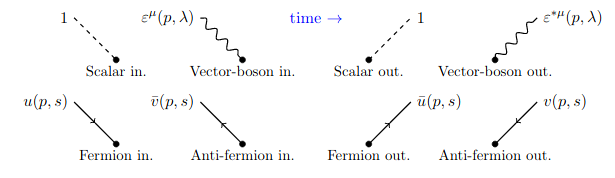
\includegraphics[width=0.8\textwidth]{intfin.png}
        \end{figure}
    \item For internal lines which connect two vertices, we put in the propagator $i\Delta$.
        These are:
        \begin{figure}[H]
            \centering
            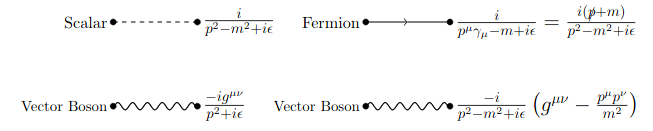
\includegraphics[width=0.8\textwidth]{props.png}
        \end{figure}
    \item For a given process, draw all possible diagrams (to a given order in your perturbative expansion) matching the external states and translate it into an amplitude $-i\mathcal{M}$ by summing over them and writing their contributions with the above prescriptions of factors for internal and external lines, and vertices.
        Impose momentum conservation on each vertex to fix the momenta of propagators as much as possible.
\end{itemize}

\chapter{Standard Model Overview}
\section{Path Integrals Conclusion}
It can be shown that all diagrams at first order in our perturbative expansion have the momenta of propagaotrs fixed in terms of the momenta of external states. 
The next order does not and there's internal momenta which we have to integrate over. 
These are the rules, but one only really learns how to use them with examples. 
Finally, we can take the invariant matrix element $-i\mathcal{M}$ and find the cross-section. 
For two particles collding and producing $n$ particles, we have
\begin{align}
    \sigma &= \frac{1}{|\vec{v}_a-\vec{v}_b|2E_{\vec{p}_a}2E_{\vec{p}_b}} \int \left(\prod_{i=1}^n\frac{d^3\vec{p}_i}{2E_{\vec{p}_i}(2\pi)^3}\right)(2\pi)^4\delta^4\left(p_a+p_b0\sum_{i=1}^np_i\right)|\mathcal{M}|^2,
\end{align}
where $\vec{v}=\vec{p}/E_{\vec{p}}$.
The terms inside the inregral except for $\mathcal{M}$ constitute the \textbf{Lorentz Invariant Phase Space}, sometimes this will be called \lips, whereas the factors out front are related to our normalisation of states $\langle\vec{p}'|\vec{p}\rangle$. 
On the other hand, a decay rate in the particle's rest frame is
\begin{align}
    \Gamma &= \frac{1}{2M_a}\int \prod_i \frac{d^3\vec{p}_i}{2E_{\vec{p}_i}(2\pi)^3}(2\pi)^4\delta^4\left(p_a-\sum_{i=1}^n p_i\right)|\mathcal{M}|^2,
\end{align}
with $p_a$ the four-momenta of the decaying particle. 
So at last our trip from action to observables is done. 

A number of useful relations for the square of the matrix elements when we sum over spins are:
\begin{align}
    \sum_s u(\vec{p},s)\bar{u}(\vec{p},s) &= \cancel{p}+m, & \sum_{\lambda}\e_\mu(\vec{p},\lambda)\e_\nu^*(\vec{p},\lambda)&=-g_{\mu\nu}\,(m=0), \\
    \sum_s v(\vec{p},s)\bar{v}(\vec{p},s) &= \cancel{p}-m, & \sum_\lambda \e_\mu(\vec{p},\lambda)\e_\nu^*(\vec{p},\lambda) &= \frac{p_\mu p_\nu}{m^2}-g_{\mu\nu},
\end{align}
and since $(\gamma^0)^\dagger = \gamma^0$, $(\gamma^\mu)^\dagger \gamma^0 = \gamma^0\gamma^\mu$, we have, for example, 
\begin{align}
    (\bar{u}\gamma^\mu v)^* &= v^\dagger (\gamma^\mu)^\dagger(\gamma^0)^\dagger u = v^\dagger \gamma^0\gamma^\mu u = \bar{v}\gamma^\mu u.
\end{align}


\section{Gauge Groups}
The Standard Model is formed under the principles of gauge theory. 
The group of the Standard Model is SU(3)$_c\otimes$SU(2)$_L\otimes$U(1)$_Y$, representing colour triplets, weak isospin doublets, and hypercharge respectively.
SU(3)$_c$ is the gauge group of colour (QCD), and the rest of the SM group is the electroweak theory which can be approximately split into the weak isospin and hypercharge, although not quite, and will result in electromagnetism after introducing the Higgs mechanism later. 
Let's overview how each gauge group is set up in terms of its bosons and generators:
\begin{table}[H]
    \centering
    \begin{tabular}{r|llc}
        \hline\hline
        & \textbf{Color} & \textbf{Weak Isospin} & \textbf{Hypercharge} \\
        \hline\hline 
        \textbf{Group:} & SU(3)$_c$ & SU(2)$_L$ & U(1)$_Y$ \\
        \textbf{Bosons:} & $\tensor{G}{_\mu^a},a=1\to8$ & $\tensor{W}{_\mu^I},I=1\to3$ & $B_\mu$ \\
        \textbf{Generators:} & $\frac{g_s}{2}T_a$ & $\frac{g}{2}\sigma_I$ & $Q_Y g'\mathbb{I}$ \\
        \hline\hline
    \end{tabular}
\end{table}
Here $g_s,g,g'$ are the couplings of colour, weak, and hypercharge respectively. 
The matrices $T_a$ and $\sigma_I$ can be taken to be the Gell-Mann and Pauli matrices respectively, with the normalisations $\text{Tr}(T_aT_b) = 2\delta_{ab}$ and $\text{Tr}(\sigma_I\sigma_J) = 2\delta_{IJ}$.
The field strengths for the gauge bosons transform in the adjoint representation and are defined as:
\begin{align}
    G_{\mu\nu} &= \p_\mu \tensor{G}{_\nu^a}T_a - \p_\nu\tensor{G}{_\mu^a}T_a + \frac{ig_s}{2}\left[\tensor{G}{_\mu^a}T_a,\tensor{G}{_\nu^b}T_b\right], \\
    W_{\mu\nu} &= \p_\mu \tensor{W}{_\nu^I}\sigma_I - \p_\nu\tensor{W}{_\mu^I}\sigma_I + \frac{ig}{2}\left[\tensor{W}{_\mu^I}\sigma_I,\tensor{W}{_\nu^J}\sigma_J\right],  \\
    B_{\mu\nu} &= \p_\mu B_\nu - \p_\nu B_\mu.
\end{align}
Gauge bosons couple to matter through the covariant derivative. 
We can simplify this and select certain terms for different interactions, so we only use terms appropriate, (e.g. we would not use the colour term for leptons), but in its full form for the SM, it is defined as
\begin{align}
    D_\mu &= \p_\mu + i\frac{g_s}{2}\tensor{G}{_\mu^a}T_a + i\frac{g}{2}\tensor{W}{_\mu^I}\sigma_I + ig'Q_Y.
\end{align}
For example, we would need this full derivative when dealing with left-handed quarks.


\chapter{Standard Model Overview Contd.}
\section{Matter}
Matter can be defined by fields that are charged under the SM gauge groups, i.e. fermions and the Higgs doublet. 
First, we remind ourselves of the definitions for chirality:
\begin{align}
    \gamma_5 &= i\gamma^0\gamma^1\gamma^2\gamma^3, & P_L &\equiv\frac{1-\gamma_5}{2}, & P_R &\equiv \frac{1+\gamma_5}{2},
\end{align}
where $P_{L,R}$ are the left/right-handed projectors. 
These projections are useful because it commutes with Lorentz transformations, i.e.
\begin{align}
    [\gamma_5,[\gamma_\mu,\gamma_\nu]] = 0.
\end{align}
So we can define the left- and right-handed components of the fermion fields by projecting using the above, which will remain invariant after a Lorentz transformation. 
The fermion fields (and Higgs) we then have are
\begin{table}[H]
    \centering
    \begin{tabular}{c|c|c|c|c|c|c}
        \hline\hline
        Gauge Group & $q_L$ & $u_R$ & $d_R$ & $l_L$ & $e_R$ & $H$ \\
        \hline\hline
        SU(3)$_c$ & 3 & 3 & 3 & - & - & - \\
        SU(2)$_L$ & 2 & - & - & 2 & - & 2 \\
        U(1)$_Y$  & $\frac16$ & $\frac23$ & $-\frac13$ & $-\frac12$ & $-1$ & $\frac12$\\
        \hline\hline
    \end{tabular}
\end{table}

\section{Lagrangian}
As we've emphasised so far, the spacetime integral of the Lagrangian dictates the evolution of the system and possible outcomes; therefore it is the central construction from which we can derive observables.
The construction of the Lagrangian of the Standard Model follows two rules: \emph{Lorentz and gauge invariance.}
These symmetries imply conserved currents which form the basis of our predictions.
Using the field strength definitions, 
\begin{align}
    G_{\mu\nu} &= \p_\mu \tensor{G}{_\nu^a}T_a - \p_\nu\tensor{G}{^a_\mu}T_a + \frac{ig_s}{2}\left[\tensor{G}{_\mu^a}T_a,\tensor{G}{^b_\mu}T_b\right], \\
    W_{\mu\nu} &= \p_\mu \tensor{W}{_\nu^I}\sigma_I - \p_\nu\tensor{W}{^I_\mu}\sigma_I + \frac{ig}{2}\left[\tensor{W}{_\nu^I}\sigma_I,\tensor{W}{^J_\nu}\sigma_J\right], \\
    B_{\mu\nu} &= \p_\mu B_\nu - \p_\nu B_\mu,
\end{align}
we start by expressing the kinetic Lagrangian expressing interactions of matter and gauge bosons:
\begin{align}
    \begin{split}
        \La_{gauge} = &-\frac18\text{Tr}(G_{\mu\nu}G^{\mu\nu})-\frac18\text{Tr}(W_{\mu\nu}) - \frac14B_{\mu\nu}B^{\mu\nu} \\
                      &+ \sum_{\psi_L} i\bar{\psi}\gamma^\mu D_\mu\psi_L + \sum_{\psi_R}i\bar{\psi}\gamma^\mu D_\mu \psi_R + D^\mu H^\dagger D_\mu H.
    \end{split}
\end{align}
However, this Lagrangian does not include mass terms, which we will come onto later with the Higgs mechanism.
We have a first guess of the Higgs potential to help introduce masses as the Mexican hat potential,
\begin{align}
    V(H) &= -m_H^2H^\dagger H + \lambda(H^\dagger H)^2.
\end{align}
From this, we can eventually arrive at the Yukawa interaction which will introduce fermion masses:
\begin{align}
    \La_{Yuk} &= -\sum_{\text{\tiny gauge inv.}} \left(Y\bar{\psi}_L H\psi_R + Y\bar{\psi}_L\tilde{H}\psi_R\right) + h.c. \\
              &= -Y_u\bar{q}_L\tilde{H}u_R - Y_d\bar{q}_L Hd_R - Y_e\bar{l}_L He_R + h.c., \\
    \tilde{H} &= i\sigma_2 H^* = \begin{pmatrix} 0 & 1 \\ -1 & 0 \end{pmatrix}H^*,
\end{align}
where we have introduced $\tilde{H}$ to protect the conservation of hypercharge where $H$ would not.
We can now put everything together for the final SM Lagrangian:
\begin{align}
    \begin{split}
        \La_{SM} = &-\frac18\text{Tr}(G_{\mu\nu}G^{\mu\nu}) - \frac18\text{Tr}(W_{\mu\nu}W^{\mu\nu}) - \frac14B_{\mu\nu}B^{\mu\nu} \\
                   &+ \sum_{\psi_L}i\bar{\psi}\gamma^\mu D_\mu\psi_L + \sum_{\psi_R} i\bar{\psi}\gamma^\mu D_\mu \psi_R + D^\mu H^\dagger D_\mu H \\
                   &- Y_u\bar{q}_L\tilde{H}u_R - Y_d\bar{q}_LHd_R - Y_e\bar{l}_LHe_R + h.c. \\
                   &+ m_H^2 H^\dagger H - \lambda(H^\dagger H)^2.
    \end{split}
\end{align}
This is the final result for a single generation of fermion. 
Eventually, we would have to add another index onto matter fields to sum over the three currently-known generations of particles, i.e. $u_R^i = (u_R^1,u_R^2,U_R^3)$.
This will cause us to move from Yukawa coupling numbers $Y$ to Yukawa $3\times3$ matrices, which introduces other phenomena later.

\section{Conservation Laws}
We have several conservation laws in the Standard Model. 
Through conserved currents, we say the charges are conserved over interactions. 
In addition, \textbf{Baryon number} is conserved, defined as
\begin{align}
    Q_B(q_L,u_R,d_R) &= \frac13(q_L,u_R,d_R).
\end{align}
Similarly, each generation of lepton has its own conservation, i.e. \textbf{Electron number}, \textbf{Muon number} are conserved, including their neutrinos in the count. 

\chapter{Deep Inelastic Scattering and Partons}
Quarks and gluons, known together as partons, are no observed as final states in experiments, yet are claimed to be components of mesons and baryons. 
What evidence is there then to this? 
We look to deep inelastic scattering and the parton model for an explanation.

Consider shooting electrons at protons at high CoM energy, $s\gg m_P^2\approx 1\,$GeV$^2$.
At these energies, electrons can probe the internal structure of the proton and `catch' partons behaving as free particles inside the proton. 
This parton will receive a large momentum transfer and break away from the proton such that, after further hadronisation to conserve colour, the proton has 'broken' into various other hadrons. 
\begin{figure}[H]
    \centering
    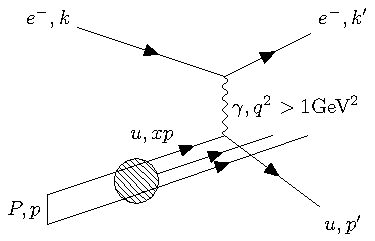
\includegraphics[scale=1.2]{dis.pdf}
\end{figure}
To see how if this agrees with experimental data, let's consider the scattering at a partonic level, specifically choosing a $u$ quark and the scattering $e+u\to e+u$.
Let's assume the $u$ quark carries a fraction $x$ of the total momentum of the proton, then the partonic process is
\begin{align}
    -i\hat{\mathcal{M}} &= ie\bar{u}_e(k')\gamma_\mu u_e(k)\frac{-ig^{\mu\nu}}{q^2}\left(-i\frac{2e}{3}\right)\bar{u}_u(p')\gamma_\nu u_u(xp),
\end{align}
with $q=k-k'=p'-xp$ and we use the `hat' to denote partonic quantities. 
Recall the formula for the cross-section, which in this case we can simplify a bit since we have \emph{relativistic particles} (we take $q^2\gg m_i^2$),
\begin{align}
    d\hat{\sigma} &= \frac12 \frac{1}{2|\vk|2x|\vec{p}|} \frac{d^3\vec{p}'\,d^3\vk'}{2|\vk'|(2\pi)^32|\vec{p}'|(2\pi)^3}|\hat{\mathcal{M}}|^2 (2\pi)^4 \delta^4(xp+k-p'-k').
\end{align}
If one works on the phase space for the final parton, 
\begin{align}
    \begin{split}
        (2\pi)^4\delta^4(xp+q-p')\frac{d^3\vp'}{(2\pi)^32|\vp'|} &= \delta(x|\vp|+q^00|x\vp+\vec{q}|)\frac{2\pi}{2|x\vp+\vec{q}|} \\
                                                                 &= \frac{\pi}{p\cdot p'}\delta\left(x+\frac{q^2}{2p\cdot q}\right) = 2\pi\frac{p\cdot q}{p\cdot p'}\delta(2p\cdot qx + q^2),
    \end{split}
\end{align}
where $q=k-k'$.
We can rewrite the above for the lepton phase space by changing the variables from $|\vk|,\cos\theta$ is the CoM frame to $q^2,p\cdot q$ as
\begin{align}
    \frac{d^3\vk'}{(2\pi)^32E_{\vk'}} &= \frac{d(q^2)\,d(p\cdot q)}{4(2\pi)^2p\cdot k},
\end{align}
where we also integrated over the angle $\phi\in[0,2\pi)$ since the amplitude does not depend on it.
For the matrix element, since we do not know the spin of the particles involved, we average over incoming and sum over outgoing as
\begin{align}
    \frac{1}{2^2}\sum_{s_e,s_u}\sum_{s_e',s_u'} \hat{\mathcal{M}}\hat{\mathcal{M}}^\dagger &= \frac14 \sum_{s_e,s_u}\sum_{s_e',s_u'} \bigg|\bar{u}_e(k',s_e')\gamma_\mu u_e(k,s_e)\frac{e^2}{q^2}\frac23 \bar{u}_u(p',s_u')\gamma^\mu u_u(xp,s_u)\bigg|^2 \\
                                                                                           &= \left(\frac{2e^2}{3q^2}\right)^2 4\text{Tr}(\gamma_\mu x\cancel{p}\gamma_\nu \cancel{p}')\text{Tr}(\gamma^\mu\cancel{k}\gamma^\nu\cancel{k}') \\
                                                                                           &= \left(\frac{2e^2}{3q^2}\right)^28\left((xp\cdot k)(p'\cdot k')+(xp\cdot k')(p'\cdot k)\right) \\
                                                                                           &= \left(\frac{2e^2}{3q^2}\right)^28\left((xp\cdot k)^2+(xp\cdot k')^2\right).
\end{align} 
We then put all this together for the cross-section and find
\begin{align}
    d\hat{\sigma} &= \left(\frac{2e^2}{3q^2}\right)^2\frac{1}{2(2xp^0)(2k^0)}8\left((xp\cdot k')^2\right) \frac{d(q^2)\,d(p\cdot q)}{4(2\pi)^2p\cdot k}\frac{\pi}{p\cdot q}\delta\left(x+\frac{q^2}{2p\cdot q}\right) \\
                  &= x\left(\frac{2e^2}{3q^2}\right)^2\frac{(p\cdot k)^2+(p\cdot(k-q))^2}{8\pi p\cdot q(p\cdot k)^2}\delta\left(x+\frac{q^2}{2p\cdot q}\right)\,d(q^2)\,d(p\cdot q).
\end{align}
Now comes the part that we cannot compute: what is the probability of the photon bumping into  parton with fraction of the momentum $x$?
This is a magnitude which we cannot estimate in perturbation theory. 
Instead, we name it the \textbf{parton distribution function} $f_u(x)$ and sum over it:
\begin{align}
    \begin{split}
        d\sigma = d\hat{\sigma}f_u(x)\,dx &= \left(\frac{2e^2}{3q^2}\right)^2\frac{p\cdot k}{4\pi}\left(1+\frac{\left(p\cdot(k-q)\right)^2}{(p\cdot k)^2}\right)\,d(p\cdot q)xf_u(x)\,dx \\
                                          &= \frac{e^2}{8\pi}\frac{s}{q^4}\left(\frac{2e}{3}\right)^2\left(1+(1-y)^2\right)\,dy\,xf_u(x)\,dx,
    \end{split}
\end{align}
where we used the Dirac delta to set
\begin{align}
    x &= -\frac{q^2}{(2p\cdot q)}, & s &= (p+k)^2\approx 2p\cdot k,
\end{align}
and found appropriate to change variable from $p\cdot q$ to variable $y=\frac{p\cdot q}{p\cdot k}$.
Finally we know it's not only the $u$ quark in the proton but also the $d$, so we add it up too:
\begin{align}
    d\sigma_{eP\to eX} &= \frac{e^2}{8\pi}\frac{s}{q^4}\left(1+(1-y)^2\right)\,dy\,\left[\left(\frac{2e}{3}\right)^2f_u(x) + \left(\frac{-e}{3}\right)^2f_d(x)\right]\,dx,
\end{align}
where by $eX$ in the final state, we sum over all possible products of the collision, termed \emph{inclusive.}
We do not know a priori $f_{u,d}(x)$, but this can still be a predictive results which can be tested against data.
The general cross-section without assuming anything about the components of the proton, only using electromagnetic gauge invariance, reads
\begin{align}
    d\sigma_{eP\to eX} &= \frac{e^4}{4\pi}\frac{s}{q^4}\left(xy^2F_1(x,y) + (1-y)F_2(x,y)\right)\,dx\,dy,
\end{align}
where $F_{1,2}$ arbitrary functions. 
Even if we start from arbitrary parton distribution functions, we cannot obtain arbitrary $F_{1,2}$, since one $f$ only depends on $x$. 
Expressed in terms of $F_{1,2}$, the conditions that follow from our quark description read
\begin{align}
    F_2(x,y) &= 2xF_1(x) = \sum_i Q_i^2 xf_i(x),
\end{align}
with $Q_i$ the charge of the parton in units of $e$ ($\frac23,-\frac13$ for $u,d$).
This relation is known as the Callan-Gross equation. 
The fact that the functions $F_{1,2}$ depend only on $x$ is knon as Bjorken scaling and a way to test it is to extract $F_{1,2}$ from experiment and plot them for fixed $x$ and varying $y$; if they do not change, the Callan-Gross relation holds and the quark model prediction is right.

\chapter{PDFs and Hadronic vs Partonic}
Studying deep inelastic scattering showed that the cross-section of the process $eP\to eX$ (where $X$ represents anything that can be produced) can be expressed as an integral over the partonic process times a function $f(x)$ of the fraction of momentum $x$, i.e.
\begin{align}
    \int d\sigma_{eP\to eX} &= \int \sum_i f_i(x)\,d\sigma_{ei\to ei}\,dx.
\end{align}
These functions $f$ are called Parton Distribution Functions and their extraction from experiment (we cannot compute them) provides a window into the proton's inner structure. 
We

\chapter{Quantum Chromodynamics}
\begin{figure}[H]
    \centering
    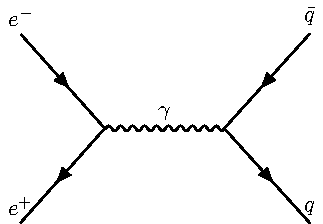
\includegraphics{epq.pdf}
    \begin{align}
        -i\mathcal{M} &= \bar{\nu}_e(ie\gamma_\nu)u_e\frac{-ig^{\mu\nu}}{s}\bar{u}_q(-ieQ_{q})\gamma_\nu v_q
    \end{align}
    \vspace{-40pt}
\end{figure}
Here, $s = (p_{e^-} + p_{e^+})^2$. 
We then have the differential cross-section:
\begin{align}
    d\sigma &= \frac14\sum_{spin} |\mathcal{M}| (2\pi)^2 \delta^2(p_{e^+}+p_{e^-}-p_{q}-p_{\bar{q}}) \frac{d^3p_q\,d^3p_{\bar{q}}}{(2\pi)^62E_{p_q}E_{p_{\bar{q}}}}
\end{align}
The extra terms here are to integrate over \textbf{Lorentz Invariant Phase Space.}
We want to reduce this, however, such that we get rid of the $\delta$ functions for convenience. 
\begin{align}
    d\textbf{LIPS} &= \frac{1}{(2\pi)^2} \delta(\sqrt{s}-E_{p_q}-E_{p_{\bar{q}}})\delta^3(-p_{q}-p_{\bar{q}}) \frac{d^3p_q\,d^3p_{\bar{q}}}{2E_{p_q}2E_{p_{\bar{q}}}} \\
                 &= \frac{1}{(2\pi)^2} \delta(\sqrt{s}-2E_{p_q})\frac{d^3p_{q}}{4E_{p_q}^2} \\
                 &= \frac{1}{(2\pi)^2} \delta(\sqrt{s}-2E_{p_q})\frac{d\Omega\,p_q^2\,dp_q}{4E_{p_q}^2}
\end{align}
A useful trick for simplifying these $\delta$ functions is
\begin{align}
    \delta(f(x)) &= \frac{1}{|f'(x)|}\delta(x-x_0).
\end{align}
So now we can use this on the modulus of the momenta:
\begin{align}
    \sqrt{s} &- 2E_{p_q} = 0 \\
    E_{p_q}^2 &= m^2 + p_q^2 = \frac{s}{4} \\
    |p_q|^2 &= \frac{s-4m^2}{4}
\end{align}
Back to our $\lips$:
\begin{align}
    \lips &= \frac{1}{(2\pi)^2} \frac{1}{|2p_q/E_{p_q}|} \frac{d\Omega\, p_q^2\,dp_q}{4E_{p_q}^2} \delta(p_q-\sqrt{\frac{s-4m^2}{4}}) \\
          &= \frac{d\Omega}{(2\pi)^2}\frac{|p_q|}{8E_{p_q}} = \frac{d\Omega}{(2\pi)^2}\frac{\sqrt{s-4m^2}}{8\sqrt{s}}
\end{align}

\chapter{Electroweak Interactions}
Spontaneous symmetry breaking induces SU(2)$_L\otimes$U(1)$_Y\to$U(1)$_{EM}$.
We have the Higgs potential for this as
\begin{align}
    V(H) &= -m_H^2H^\dagger H + \lambda(H^\dagger H)^2, \\
    \langle0|H|0\rangle &= \begin{pmatrix} 0 \\ \frac{v}{\sqrt{2}}\end{pmatrix},
\end{align}
producing a Mexican hat potential with a VEV shown above. 
This Higgs mechanism allows us to generate gauge boson masses for the $W^\pm,Z$ bosons. 
For the vacuum value, we have
\begin{align}
    D_\mu\langle H\rangle &= i\begin{pmatrix} \frac{g'}{2}B_\mu + \frac{g}{2}W_\mu^3 & \frac{g}{2}\left(W^1_\mu - iW_\mu^2\right) \\ \frac{g}{2}\left(W_\mu^1+iW_\mu^2\right) & \frac{g'}{2}B_\mu - \frac{g}{2}W_\mu^3\end{pmatrix} \begin{pmatrix} 0 \\ \frac{v}{\sqrt{2}} \end{pmatrix} = \frac{iv}{\sqrt{2}}\begin{pmatrix} \frac{g}{2}(W_\mu^1-iW_\mu^2) \\ \frac{g'}{2}B_\mu - \frac{g}{2}W_\mu^2\end{pmatrix}.
\end{align}
The kinetic term for the vec of the Higgs is the modulus of this, i.e.
\begin{align}
    D_\mu\langle H\rangle^\dagger D^\mu\langle H\rangle &= \frac{v^2}{2}\left(\frac{g^2}{4}|W_\mu^1-iW_\mu^2|^2 + \left(\frac{g'}{2}B_\mu - \frac{g}{2}W_\mu^3\right)^2\right).
\end{align}
The gauge fields $W^i,B$ do not themselves have mass terms, but from the above, we can introduce linear combinations of them which will:
\begin{align}
    W_\mu^\pm &= \frac{1}{\sqrt{2}}\left(W_\mu^1\mp iW_\mu^2\right) & \frac{g}{2}W_\mu^3 - \frac{g'}{2}B_\mu &= \frac{\sqrt{g^2+g'^2}}{2}Z_\mu,
\end{align}
so we now have the $W^\pm,Z$ fields corresponding to the real observable bosons, where the massless photon field $A_\mu$ comes from the relation
\begin{align}
    \begin{pmatrix} Z_\mu \\ A_\mu \end{pmatrix} &= \begin{pmatrix} \cos\theta_w & -\sin\theta_w \\ \sin\theta_w & \cos\theta_w\end{pmatrix}\begin{pmatrix} W_\mu^3 \\ B_\mu^3\end{pmatrix}, \quad \cos\theta_w = \frac{g}{\sqrt{g^2+g'^2}}.
\end{align}
We can feed these fields back into Eq. (10.4) as
\begin{align}
    D_\mu\langle H\rangle^\dagger D^\mu\langle H\rangle &= \frac{v^2}{2}\left(\frac{g^2}{2}W_\mu^+W^{-\mu} + \frac{g^2}{4\cos^2\theta_w}Z_\mu Z^\mu\right),
\end{align}
which produce mass terms in the Lagrangian appearing as
\begin{align}
    \La_M &= M_W^2W_\mu^+ W^{-\mu} + \frac12 M_Z^2 Z_\mu Z^\mu.
\end{align}
We can read the masses out from this, yielding
\begin{align}
    M_W &= \frac{gv}{2} = 80\,\text{GeV}, & M_Z &= \frac{gv}{2\cos\theta_w} = 91\,\text{GeV}.
\end{align}
From all this, we can then write our lengthy descriptions of $D_\mu$ to see the full self-interactions of these bosons where we will see three- and four-point vertices emerges. 
It is then convenient to address the coupling of electroweak bosons to fermions. 
The electromagnetic coupling is the U(1) symmetry left over from SSB, and we define its coupling strength as 
\begin{align}
    e &= g\sin\theta_w,
\end{align}
where the only gauge invariant combination of the weak isospin and hypercharge charges we had previously is now the electric charge, given by
\begin{align}
    Q^L_{em} &= \frac{\sigma_3}{2} + Q^L_Y,\quad Q_{em}^R = Q_Y^R \\
    Q_{em} &= \left(\frac{\sigma_3}{2}+Q_Y^L\right)P_L + Q_Y^RP_R,
\end{align}
where $L,R$ denotes left- and right-handed fermions. 
It is worth noting that electromagnetism is not chiral, i.e. $Q_{em}^L = Q^R_{em}$ and there is no $\gamma_5$ term in the coupling. 
Chirality does however remain in the couplings of the $W^\pm,Z$ bosons, where $W^\pm$ bosons still only couple to left-handed fields.  

\chapter{Electroweak Boson Properties}
$W^\pm,Z$ bosons theorised in the 60s then discovered in the 80s. 
We perform electron-positron collisions to produce the $Z$ boson, with a matrix element for the reaction $e^+e^-\to Z\to\mu^+\mu^-$,
\begin{align}
    -i\mathcal{M} &= -\frac{ig}{\cos\theta_w}\bar{v}_e\gamma^\rho\left(-\frac{P_L}{2}+\sin^2\theta_w\right)u_e\frac{ig_{\rho\nu}+i\frac{p_\rho^Zp_\nu^Z}{M_Z^2}}{s-m_Z^2+i\e}\left(-\frac{ig}{\cos\theta_w}\right)\bar{u}_{\mu^-}\gamma^\nu\left(-\frac{P_L}{2}+\sin^2\theta_w\right)v_{\mu^+},
\end{align}
with $s=(p_{e^+}+p_{e^-})^2$.
Initially, this was run with $s=90\,$GeV, where the Z propagator seems to blow up. 
When the particle is produced on resonance, i.e. $s=M_Z^2$, we have to reconsider what's going on. 
In this regime, the Z boson is no longer a virtual short-distance mediator, but must be consider a possible final state itself, if the particle is stable. 
If the Z boson is an unstable particle, with a short lifetime, we need to modify the particle propagator to say how it evolves.

If we modify the propagator's denominator as $M_Z\to M_Z-\frac{i}{2}\Gamma_Z$ with $\Gamma_Z$ the total decay width of the Z boson. 
This extram imaginary part in the action for the particle gives a time evolution, and hence an exponential decay for its probability. 
The resulting propagator and cross-section scales as
\begin{align}
    d\sigma &\propto \frac{1}{|s-M_Z^2+i\Gamma_ZM_Z - \Gamma_Z^2/4|^2} \approx \frac{1}{(s-M_Z^2)^2+\Gamma_Z^2M_Z^2}.
\end{align}
This is called a Breit-Wigner distribution and looks like a peak at $s=M_Z^2$, which is sharper for smaller $\Gamma_Z/M_Z$. 
We call a small (large) $\Gamma_Z/M_Z$ a narrow (broad) resonance.
In the case of a well-defined peak, the Narrow Width Approximation applies and we can compute the cross-section as the exchange of an on-shell Z which implies production and decay are factorised which reads
\begin{align}
    \sigma_{N.W.A} &= \frac{12\pi s}{M_Z^2} \frac{\Gamma(Z\to e^+e^-)\Gamma(Z\to\mu^+\mu^-)}{(s-M_Z^2)^2+M_Z^2\Gamma_Z^2}.
\end{align}
We can use this to break down the calculation into smaller pieces and look for different decays and reconstruct couplings of the Z boson. 
Let's focus on one decay in particular: $e^+e^-\to Z\to\bar{\nu}\nu$.
The interaction term can be derived from the kinetic term, reading
\begin{align}
    \La_{int} &= i(\bar{l}_L\gamma^\mu D_\mu l_L) = i\bar{\nu}\frac{igZ^\mu}{\cos\theta_w}\gamma_\mu\left(\frac{(\sigma_3)_{11}}{2}P_L - \sin^2\theta_w Q_{em}^\nu\right)\nu + \cdots, \\
              &= -\frac{gZ_\mu}{2\cos\theta_w}\bar{\nu}\gamma^\nu P_L\nu + \cdots, \\
    -i\mathcal{M}_{Z\to\bar{\nu}\nu} &= \e^\mu(p_Z,\lambda)\bar{u}_\nu(p_\nu,s_\nu)\frac{-ig}{2\cos\theta_w}\gamma_\mu P_Lv_\nu(p_{\bar{\nu}},s_{\bar{\nu}}).
\end{align}
For computing the rate, we average over the initial states for the polarisations $\lambda=\pm1,0$, and we sum over all possible final states, i.e.
\begin{align}
    \frac13 \sum_{\lambda} \sum_{s_\nu s_{\bar{\nu}}} \mathcal{M}\mathcal{M}^* &= \frac13 \frac{g^2}{4\cos^2\theta_w} \sum_\lambda \sum_{s_\nu s_{\bar{\nu}}} \e_\mu\e_\rho^* \bar{u}\gamma^\mu P_L vv^\dagger P_L^\dagger (\gamma^\rho)^\dagger (\gamma^0)^\dagger u, \\
                                                                               &= \frac13 \frac{g^2}{4\cos^2\theta_w} \sum_\lambda \sum_{s_\nu s_{\bar{\nu}}} \e_\mu\e_\rho^* \bar{u}\gamma^\mu v\bar{v}\gamma^\rho P_L u \\
                                                                               &= \frac13 \frac{g^2}{4\cos^2\theta_w} \left(\frac{p^\mu_Z p^\rho_Z}{M_Z^2} - \eta^{\mu\rho}\right)\text{Tr}\left(\gamma_\mu P_L\cancel{p}_{\bar{\nu}}\gamma_\rho P_L\cancel{p}_\nu\right).
\end{align}
Now using the fact that we can bring one $P_L$ to the other and $P_L^2=P_L$, with the relation
\begin{align}
    \text{Tr}(\gamma_\mu\gamma_\alpha\gamma_\rho\gamma_\beta P_R) = 2\left(\eta^{\mu\alpha}\eta^{\rho\beta}+\eta^{\mu\beta}\eta^{\rho\beta}-\eta^{\rho\mu}\eta^{\alpha\beta}+i\e^{\mu\alpha\rho\beta}\right),
\end{align}
we can find that
\begin{align}
    \begin{split}
        &\frac13 \frac{g^2}{4\cos^2\theta_w}\left(\frac{p_Z^\mu p_Z^\rho}{M_Z^2}-\eta^{\mu\rho}\right)\text{Tr}(\gamma_\mu P_L\cancel{p}_{\bar{\nu}}\gamma_\rho P_L\cancel{p}_\nu) \\
        =&\frac{g^2}{6\cos^2\theta_w}\left(\frac{p_Z^\mu p_Z^\rho}{M_Z^2}-\eta^{\mu\rho}\right)\left((p_{\bar{\nu}})_\mu(p_\nu)_\rho + (p_{\bar{\nu}})_\rho(p_\nu)_\mu - \eta^{\rho\mu}p_{\bar{\nu}}\cdot p_\nu + i\e^{\mu\alpha\rho\beta}(p_{\bar{\nu}})_\alpha(p_\nu)_\beta\right) \\
        =&\frac{g^2}{6\cos^2\theta_w}\left(2\frac{p_Z\cdot p_\nu p_Z\cdot p_{\bar{\nu}}}{M_Z^2} + p_\nu\cdot p_{\bar{\nu}}\right),
    \end{split}
\end{align}
where given that $\e^{\mu\nu\rho\sigma}$ is fully antisymmetric, the contraction with the averaged $\e\e^*$ cancels. 
Now working in phase space for the CoM frame, we get
\begin{align}
    \frac{d^3\vec{p}_\nu\,d^3\vec{p}_{\bar{\nu}}}{2|\vec{p}_\nu|2|\vec{p}_{\bar{\nu}}|(2\pi)^6} (2\pi)^4\delta(p_Z-p_\nu-p_{\bar{\nu}}) &= \frac{d^3\vec{p}_\nu}{4|\vec{p}_\nu|^2(2\pi)^2}\delta(M_Z-|p_\nu|-|p_\nu|) \\
                                                                                                                                        &= \frac{\sin\theta\,d\theta\,d\phi}{4(2\pi)^2}\delta(M_Z-2|\vec{p}_\nu|)\,d|\vec{p}_\nu|\\
                                                                                                                                        &= \frac{\sin\theta,d\theta\,d\phi}{8(2\pi)^2}.
\end{align}
The product of the momenta $p_i$ in the matrix element squared then read
\begin{align}
    p_\nu\cdot p_{\bar{\nu}} &= |\vec{p}_\nu||\vec{p}_{\bar{\nu}}| - \vec{p}_\nu\cdot \vec{p}_{\bar{\nu}} = 2|\vec{p}_\nu|^2 = \frac{M_Z^2}{2}, & p_\nu\cdot p_Z &= M_Z|\vec{p}_\nu| = \frac{M_Z^2}{2},
\end{align}
where we have used four-momentum conservation and in that the neutrinoes share the Z mass. 
Finally, overall for the decay width, we get
\begin{align}
    \Gamma_{Z\to\nu\bar{\nu}} &= \frac{1}{2M_Z}\int \frac{d^3\vec{p}_\nu\,d^3\vec{p}_{\bar{\nu}}}{2|\vec{p}_\nu|2|\vec{p}_{\bar{\nu}}|(2\pi)^6} (2\pi)^4\delta(p_Z-p_\nu-p_{\bar{\nu}})\frac13\sum_{\lambda}\sum_{s_\nu s_{\bar{\nu}}} \mathcal{M}\mathcal{M}^* \\
                              &= \frac{1}{2M_Z}\frac{1}{8\pi}\frac{g^2}{6\cos^2\theta_w}M_Z^2 = \frac{g^2 M_Z}{96\pi \cos^2\theta_w}.
\end{align}
How many neutrino flavours are there though?
If we say there are $N_\nu$, then
\begin{align}
    \Gamma_{Z\to\sum_i\bar{\nu}_i\nu_i} &= \frac{g^2 N_\nu M_Z}{96\pi\cos^2\theta_w}.
\end{align}
We can compare this to experiment to find $N_\nu$.
This isn't the easiest thing in experiment to pick up as neutrinos escape detection, but we can extract this from the total width of the Z boson, and subtracting all known decays. 
What is leftover, is the decay to neutrinos. 
Comparing this to Eq. (11.18), we find that 
\begin{align}
    N_\nu &= 2.9840 \pm 0.0082,
\end{align}
which is a pretty clear indication that there are 3 neutrino flavours. 

The W boson cannot be produced like the Z that is `in the s channel', but we can produce $\pm$ pairs via, e.g., $e^+e^-\to\gamma/Z\to W^+W^-$.
The condition for this is, however, stricter than for the Z boson. 
We are now producing two W bosons where before we only had to produce the one Z boson, so we must have a CoM energy $s>2M_W$.
It is also worth nothing that we can study the chiral structure of the $W^\pm,Z$ couplings through the angular dependence of their decays. 
Another prediction from the SM is the mass ratio of the $W^\pm,Z$ bosons. 
These masses are directly related through the weak-mixing $\cos\theta_w$.
Experimentally, we can find this ratio to be
\begin{align}
    \frac{M_W^2}{\cos^2\theta_w M_Z^2} = 1.0010\pm0.0050,
\end{align}
where the SM predicts this to be eaxctly one. 
We have another confirmation of the validity of the SM. 




\end{document}













